\section{\qub{}}\label{sec:qub}
% (10 min)

\begin{frame}
  \frametitle{\qub{}}
  \begin{center}
    \begin{itemize}
    \item Quill: {\color{blue}Qu}al{\color{blue}i}fied types + {\color{blue}l}inear {\color{blue}l}ogic\\
    \item \qub{}: {\color{blue}Qu}alified types + logic of {\color{blue}b}unched implications 
    \end{itemize}
  \end{center}
\end{frame}

\begin{frame}
  \frametitle{\qub{}: Types and Predicates}
  \begin{center}
      \begin{minipage}{0.65\linewidth}
    \begin{flalign*}
      \text{Types}\ \ \  \tau, \upsilon, \phi         &::= t \mid \iota \mid \tau \rightarrow \tau\\
      &\text{where}\qquad \rightarrow \in \{\tightoverset{\scalebox{0.5}{!}}{\sepimp}, \sepimp, \tightoverset{\scalebox{0.5}{!}}{\shimp}, \shimp \}\\
      \text{Predicates}\ \ \        \pi,\omega        &::= \Un{\tau} \mid \ShFun{\phi} \mid \SeFun{\phi} \mid \tau \geq \tau' %\\
      % { \color{battleshipgrey}
      % \text{Qualified Types}\ \ \     \rho            &::= \tau \mid \pi => \rho \\
      % \text{Type schemes}\ \ \        \sigma          &::= \rho \mid \forall t. \sigma
      % }
    \end{flalign*}
  \end{minipage}

  \begin{itemize}
  \item $\SeFun{\phi}$: $\phi$ is a function that is separate from its argument
  \item $\ShFun{\phi}$: $\phi$ is a function that is in sharing with its argument
  \item $\Un{\tau}$: $\tau$ does not have resources or they can be copied/dropped easily
  \end{itemize}
  \end{center}
\end{frame}


\begin{frame}
  \frametitle{\qub{}: Types and Predicates}
  \begin{center}
    \begin{minipage}{0.65\linewidth}
      \begin{flalign*}
        \text{Types}\ \ \  \tau, \upsilon, \phi         &::= t \mid \iota \mid \tau \rightarrow \tau\\
        &\text{where}\qquad \rightarrow \in \{\tightoverset{\scalebox{0.5}{!}}{\sepimp}, \sepimp, \tightoverset{\scalebox{0.5}{!}}{\shimp}, \shimp \}\\
        \text{Predicates}\ \ \        \pi,\omega        &::= \Un{\tau} \mid \ShFun{\phi} \mid \SeFun{\phi} \mid \tau \geq \tau' %\\
        % { \color{battleshipgrey}
        % \text{Qualified Types}\ \ \     \rho            &::= \tau \mid \pi => \rho \\
        % \text{Type schemes}\ \ \        \sigma          &::= \rho \mid \forall t. \sigma
        % }
    \end{flalign*}
    \end{minipage}
  \begin{itemize}
  \item $\sepimp$: Function type that is separate with its argument
  \item $\shimp$: Function type that is in sharing with its argument
  \item $\tightoverset{\scalebox{0.5}{!}}{\sepimp}$, $\tightoverset{\scalebox{0.5}{!}}{\shimp}$: unrestricted versions of $\sepimp$ and $\shimp$
  \end{itemize}
  \end{center}
\end{frame}

\begin{frame}
  \frametitle{\qub{}: Expression Language}
  \begin{center}
    \begin{flalign*}
      \text{Term Variables}\ \ \  x, y, z  &\in \text{Var} \nonumber\\
      \text{Expressions}\ \ \     M, N     &::= x \\
                                           & \mid \lambda^{\sepimp}x. M \mid \lambda^{\shimp}x. M \\
                                           & \mid M N \mid \Let{x}{M}{N}\nonumber
    \end{flalign*}
    \begin{itemize}
    \item $\lambda^{\sepimp}x. M$: Argument $x$ separate from $M$
    \item $\lambda^{\shimp}x. N$: Argument $x$ sharing with $M$
    \end{itemize}
  \end{center}
\end{frame}

\begin{frame}
  \frametitle{\qub{}: Typing Environment}
  \begin{center}
    \begin{itemize}
    \item Logic of \BI{}: Contexts are trees
    \item \qub{}: Contexts generalized to graphs
    \end{itemize}
    {\small
      \begin{minipage}[c]{0.45\linewidth}
      \centering
      \tikzset{every tree node/.style={minimum width=2em},
        blank/.style={draw=none},
        edge from parent/.style=
        {draw,edge from parent path={(\tikzparentnode) -- (\tikzchildnode)}},
        level distance=1.5cm}
      \begin{tikzpicture}
        \Tree
        [.,
        [.;
        [.a:A ]
        [.b:B ]
        ]
        [.c:C ]
        ]
      \end{tikzpicture}
    \end{minipage}\hfill%
    \begin{minipage}[c]{0.45\linewidth}
      \centering
      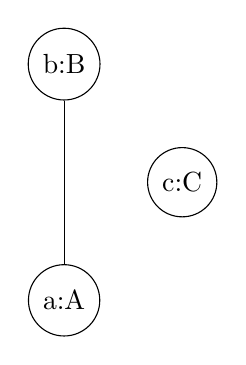
\begin{tikzpicture}
        \node[shape=circle,draw=black] (A) at (0,0) {a:A};
        \node[shape=circle,draw=black] (B) at (0,3) {b:B};
        \node[shape=circle,draw=black] (C) at (1.5,1.5) {c:C};

        \path [-] (A) edge node {} (B);
      \end{tikzpicture}
    \end{minipage}
  }
  \begin{itemize}
  \item Nodes are program objects
  \item (No) Edges represent (no) sharing
\end{itemize}
\end{center}
\end{frame}


\begin{frame}[fragile, c]
  \frametitle{\qub{}: Typing Environment}
  \begin{center}
    Sharing relation $\Psi$

    \begin{table}[h]
      \centering
      \begin{tabular}[c]{c c c}
      reflexive
      & $\forall x.\ x \mathbin{\Psi} x$
      & \raisebox{-0.4\height}{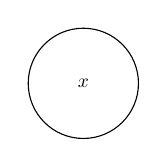
\begin{tikzpicture}[scale=0.7, fill=white, transform shape]
          \draw (0,0) circle  (1cm) node {$x$};
        \end{tikzpicture}}\\
      symmetric
      & $ \forall x, y.\ x \mathbin{\Psi} y \Rightarrow y \mathbin{\Psi} x$
      & \raisebox{-0.4\height}{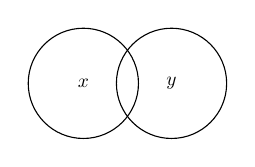
\begin{tikzpicture}[scale=0.7, fill=white, transform shape]
          \draw (0,0) circle  (1cm) node {$x$};
          \draw (1.6,0) circle  (1cm) node {$y$};
        \end{tikzpicture}}\\
      non-transitive
      & $\forall x, y, z.\ x \mathbin{\Psi} y \wedge y \mathbin{\Psi} z \not\Rightarrow x \mathbin{\Psi} z$
      & \raisebox{-0.4\height}{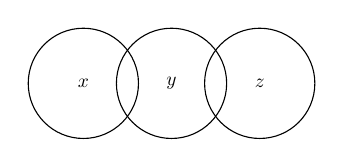
\begin{tikzpicture}[scale=0.7, fill=white, transform shape]
          \draw (0,0) circle  (1cm) node {$x$};
          \draw (1.6,0) circle  (1cm) node {$y$};
          \draw (3.2,0) circle  (1cm) node {$z$};
        \end{tikzpicture}}
      \end{tabular}
    \end{table}

\end{center}

\end{frame}

\begin{frame}
  \frametitle{\qub{}: Typing Environment}
  \begin{center}
    Flatten graphs into adjacency lists

    ``$x$ of type $\sigma$ is in sharing with $\vec{y}$''

    $(x, \sigma, \vec{y}) \in \Gamma$
    \begin{flalign*}
      \text{Typing Context}\ \ \      \Gamma,\Delta     &::= \epsilon \mid \Gamma, x^{\vec{y}}:\sigma
    \end{flalign*}
    % \begin{flalign*}
    %   \texttt{Vars}(\Gamma, x^{\vec{y}}:\tau) &= \texttt{Vars}(\Gamma) \cup \{ x \}\\
    %   \texttt{Shared}(\Gamma, x^{\vec{y}}:\tau) &= \texttt{Shared}(\Gamma) \cup \{ \vec{y} \}\\
    %   \texttt{Used}(\Gamma) &= \texttt{Vars}(\Gamma) \cup \texttt{Shared}(\Gamma)
    % \end{flalign*}
    % \begin{flalign*}
    %   (\Gamma, x^{\vec{y}}:\tau)^{[a \mapsto \vec{b}]} &= \begin{cases}
    %     a \notin \vec{y}\ \ \ \ (\Gamma^{[a \mapsto \vec{b}]}, x^{\vec{y}}:\tau)\\
    %     a \in \vec{y}\ \ \ \  (\Gamma^{[a \mapsto \vec{b}]}, x^{(\vec{y}\backslash a)\cup\vec{b}}:\tau)
    %   \end{cases}\\
    %   \Gamma^{[\vec{a} \mapsto \vec{b}]} &= (\dots((\Gamma^{[a_1 \mapsto \vec{b}]})^{[a_2 \mapsto \vec{b}]})^{\dots})^{[a_n \mapsto \vec{b}]}
    % \end{flalign*}
    % \begin{flalign*}
    %   \Gamma \circledast \Gamma' &= \Gamma \sqcup \Gamma' \qquad
    %   \texttt{if}\ \texttt{Vars}(\Gamma) \mathbin{\#} \texttt{Used}(\Gamma') \wedge \texttt{Vars}(\Gamma') \mathbin{\#} \texttt{Used}(\Gamma)\\
    %   \Gamma \varoplus \Gamma'   &= \Gamma \sqcup \Gamma' \qquad
    %   \texttt{if}\ \texttt{Used}(\Gamma) = \texttt{Used}(\Gamma')
    % \end{flalign*}
  \end{center}
\end{frame}

% \begin{frame}
%   \frametitle{\qub{}: Typing Rules}
%   \begin{center}
%     \fbox{Structural Rules}
%     {\footnotesize
%       \begin{figure}[h]\centering
%     % ID
%     \begin{minipage}{1\textwidth}
%       \begin{prooftree}
%         \AxiomC{{\color{white}$\Gamma \circledast \Delta \circledast$}} \RightLabel{[ID]}
%         \UnaryInfC{$P \mid x^{\vec{y}} : \sigma \vdash x : \sigma $}
%       \end{prooftree}
%     \end{minipage}

%     % CTR UN
%     \begin{minipage}{.55\textwidth}
%       \begin{prooftree}
%         \AxiomC{$P \mid \Gamma \circledast \Delta \circledast \Delta \vdash M : \sigma$}
%         \AxiomC{$P \vdash \Delta\ \texttt{un}$} \RightLabel{[CTR-UN]}
%         \BinaryInfC{$P \mid \Gamma \circledast \Delta \vdash M : \sigma$}
%       \end{prooftree}
%     \end{minipage}%
%     % CTR Sh
%     \begin{minipage}{.45\textwidth}
%       \begin{prooftree}
%         \AxiomC{$P \mid \Gamma \varoplus \Delta \varoplus \Delta\vdash M : \sigma$}\RightLabel{[CTR-SH]}
%         \UnaryInfC{$P \mid \Gamma \varoplus \Delta \vdash M : \sigma$}
%       \end{prooftree}
%     \end{minipage}

%     % WKN UN
%     \begin{minipage}{.50\textwidth}
%       \begin{prooftree}
%         \AxiomC{$P \mid \Gamma \vdash M : \sigma$}
%         \AxiomC{$P \vdash \Delta\ \texttt{un}$} \RightLabel{[WKN-UN]}
%         \BinaryInfC{$P \mid \Gamma \circledast \Delta \vdash M : \sigma$}
%       \end{prooftree}
%     \end{minipage}%
%     % WKN Sh
%     \begin{minipage}{.50\textwidth}
%       \begin{prooftree}
%         \AxiomC{$P  \mid \Gamma \vdash M : \sigma$} \RightLabel{[WKN-SH]}
%         \UnaryInfC{$P \mid \Gamma \varoplus \Delta \vdash M : \sigma$}
%       \end{prooftree}
%     \end{minipage}
%   \end{figure}
% }

%   \end{center}
% \end{frame}

% \begin{frame}
%   \frametitle{\qub{}: Typing Rules}
%   \begin{center}
%     \fbox{Connective Rules}
%     {\footnotesize
%       \begin{figure}[h]\centering
%     % let
%     \begin{minipage}{1\textwidth}
%       \begin{prooftree}
%         \AxiomC{$P \mid \Gamma \vdash M : \sigma$}
%         \AxiomC{$P' \mid \Gamma'_{x}, x: \sigma \vdash N: \tau$} \RightLabel{[LET]}
%         \BinaryInfC{$P \cup P' \mid \Gamma \sqcup \Gamma' \vdash (\Let{x}{M}{N}): \tau$}
%       \end{prooftree}
%     \end{minipage}
% \newline\newline\newline
%     % forall I
%     \begin{minipage}{0.50\textwidth}
%       \begin{prooftree}
%         \AxiomC{$P \mid \Gamma \vdash M: \sigma$}
%         \AxiomC{$t \notin \texttt{fvs}(\Gamma) \cup \texttt{fvs}(P)$}\RightLabel{[$\forall$ I]}
%         \BinaryInfC{$P \mid \Gamma \vdash M: \forall t. \sigma$}
%       \end{prooftree}
%     \end{minipage}%
%     % forall E
%     \begin{minipage}{0.45\textwidth}
%       \begin{prooftree}
%         \AxiomC{$P \mid \Gamma \vdash M: \forall t.\sigma$}\RightLabel{[$\forall$ E]}
%         \UnaryInfC{$P \mid \Gamma \vdash M: [\tau \backslash t] \sigma $}
%       \end{prooftree}
%     \end{minipage}
% \newline\newline\newline
%     % \Rightarrow I
%     \begin{minipage}{0.50\textwidth}
%       \begin{prooftree}
%         \AxiomC{$P, \pi \mid \Gamma \vdash M : \rho$} \RightLabel{[$\Rightarrow$ I]}
%         \UnaryInfC{$P \mid \Gamma \vdash M : \pi \Rightarrow \rho$}
%       \end{prooftree}
%     \end{minipage}%
%     % \Rightarrow E
%     \begin{minipage}{0.45\textwidth}
%       \begin{prooftree}
%         \AxiomC{$P \mid \Gamma \vdash M : \pi \Rightarrow \rho$}
%         \AxiomC{$P \vdash \pi$} \RightLabel{[$\Rightarrow$ E]}
%         \BinaryInfC{$P \mid \Gamma \vdash M: \rho$}
%       \end{prooftree}
%     \end{minipage}
% \newline\newline\newline
%     % -&> I
%     \begin{minipage}{0.45\textwidth}
%       \begin{prooftree}
%         \AxiomC{$P \Rightarrow \texttt{ShFun}\ \phi\ \ \ \ \
%           P \vdash \Gamma \geq \phi$}\noLine\def\extraVskip{-0.2pt}
%         \UnaryInfC{$P \mid \Gamma^{[\emptyset\mapsto \{x\}]},x^{\text{Vars}(\Gamma)}: \tau \vdash M : \tau'$}\RightLabel{[$\shimp$ I]}\def\extraVskip{2pt}
%         \UnaryInfC{$P \mid \Gamma \vdash \lambda^{\shimp}x. M : \phi \tau \tau'$}
%       \end{prooftree}
%     \end{minipage}%
%     % -&> E
%     \begin{minipage}{0.50\textwidth}
%       \begin{prooftree}
%         \AxiomC{$P \Rightarrow \texttt{ShFun}\ \phi$}\noLine\def\extraVskip{0pt}
%         \UnaryInfC{$P \mid \Gamma \vdash M : \phi \tau \tau'\ \ \ \ \
%           P \mid \Gamma' \vdash N : \tau$} \RightLabel{[$\shimp$ E]}\def\extraVskip{2pt}
%         \UnaryInfC{$P \mid \Gamma \varoplus \Gamma' \vdash M N : \tau'$}
%       \end{prooftree}
%     \end{minipage}
% \newline\newline\newline
%     % -*> I
%     \begin{minipage}{0.50\textwidth}
%       \begin{prooftree}
%         \AxiomC{$P \Rightarrow \texttt{SeFun}\ \phi\ \ \ \ \ P \vdash \Gamma \geq \phi$}\noLine\def\extraVskip{0pt}
%         \UnaryInfC{${\color{white}\ \ \ \ }P \mid \Gamma,x^{\emptyset}: \tau \vdash M : \tau'{\color{white}\ \ \ \ }$} \RightLabel{[$\sepimp$ I]}\def\extraVskip{2pt}
%         \UnaryInfC{$P \mid \Gamma \vdash \lambda^{\sepimp}x. M : \phi \tau \tau'$}
%       \end{prooftree}
%     \end{minipage}%
%     % -*> E
%     \begin{minipage}{0.45\textwidth}
%       \begin{prooftree}
%         \AxiomC{$P \Rightarrow \texttt{SeFun}\ \phi$}\noLine\def\extraVskip{0pt}
%         \UnaryInfC{$P \mid \Gamma \vdash M : \phi \tau \tau'\ \ \ \
%           P \mid \Gamma' \vdash N : \tau$}\RightLabel{[$\sepimp$ E]}\def\extraVskip{2pt}
%         \UnaryInfC{$P \mid \Gamma \circledast \Gamma' \vdash M N : \tau'$}
%       \end{prooftree}
%     \end{minipage}
%   \end{figure}
% }
% \end{center}

% \end{frame}

% \begin{frame}[c]
%   \frametitle{\qub{}: Typing Terms}
%   \begin{center}
%   \begin{minipage}[h]{1.0\linewidth}
%     {\tiny
%       \begin{prooftree}\def\extraVskip{6pt}
%         \AxiomC{$$}\RightLabel{[ID]}
%         \UnaryInfC{$\emptyset \mid y^{\emptyset}:\tau' \vdash y: \tau' $}

%         \AxiomC{$$}\RightLabel{[ID]}
%         \UnaryInfC{$\emptyset \mid x^{\emptyset}: \tau \vdash x: \tau$}

%         \AxiomC{$$}\RightLabel{[ID]}
%         \UnaryInfC{$\emptyset \mid f^{\emptyset}: \tau \sepimp \tau' \sepimp \upsilon \vdash f: \tau \sepimp \tau' \sepimp \upsilon $}\RightLabel{[$\sepimp$E]}
%         \BinaryInfC{$\emptyset \mid x^{\emptyset}: \tau \circledast f^{\emptyset}: \tau \sepimp \tau' \sepimp \upsilon \vdash f x: (\tau' \sepimp \upsilon)$}
%         \RightLabel{[$\sepimp$E]}

%         \BinaryInfC{$\emptyset \mid y^{\emptyset}:\tau' \circledast x^{\emptyset}:\tau \circledast f^{\emptyset}:\tau \sepimp \tau' \sepimp \upsilon \vdash f x y: \upsilon$}
%         \RightLabel{[$EXCH$]}
%         \UnaryInfC{$\emptyset \mid x^{\emptyset}:\tau \circledast y^{\emptyset}:\tau' \circledast f^{\emptyset}:\tau \sepimp \tau' \sepimp \upsilon \vdash f x y: \upsilon$}\RightLabel{[$\sepimp$ I]}
%         \UnaryInfC{$\emptyset \mid x^{\emptyset}:\tau \circledast y^{\emptyset}:\tau' \vdash \lambda^{\sepimp}f. f x y: (\tau \sepimp \tau' \sepimp \upsilon) \sepimp \upsilon$}\RightLabel{[$\sepimp$ I]}
%         \UnaryInfC{$\emptyset \mid x^{\emptyset}:\tau \vdash \lambda^{\sepimp}y. \lambda^{\sepimp}f. f x y: \tau' \sepimp (\tau \sepimp \tau' \sepimp \upsilon) \sepimp \upsilon$}\RightLabel{[$\equiv$]}
%         \UnaryInfC{$\emptyset \mid I \vdash \lambda^{\sepimp}x. \lambda^{\sepimp}y. \lambda^{\sepimp}f. f x y: \tau \sepimp \tau' \sepimp (\tau \sepimp \tau' \sepimp \upsilon) \sepimp \upsilon$}
%       \end{prooftree}
%     }
% \end{minipage}
% \end{center}

% \end{frame}

% \begin{frame}[c]
%   \frametitle{\qub{}: Typing Terms}
%   \begin{center}
%   \begin{minipage}[h]{1.0\linewidth}
%     {\tiny
%   \begin{prooftree}\def\extraVskip{6pt}
%     \AxiomC{$$}\RightLabel{[ID]}
%     \UnaryInfC{$\emptyset \mid y^{xf}: \tau' \vdash y: \tau' $}

%     \AxiomC{$$}\RightLabel{[ID]}
%     \UnaryInfC{$\emptyset \mid x^{fy}: \tau \vdash x: \tau$}

%     \AxiomC{$$}\RightLabel{[ID]}
%     \UnaryInfC{$\emptyset \mid f^{xy}: \tau \shimp \tau' \shimp \upsilon \vdash f: \tau \shimp \tau' \shimp \upsilon$}\RightLabel{[$\sepimp E$]}
%     \BinaryInfC{$\emptyset \mid x^{xy}:\tau \varoplus f^{xy}: \tau \shimp \tau' \shimp \upsilon \vdash f x: (\tau' \shimp \upsilon)$}\RightLabel{[$\shimp E$]}

%     \BinaryInfC{$\emptyset \mid y^{xf}:\tau' \varoplus x^{yf}:\tau \varoplus f^{xy}:\tau \shimp \tau' \shimp \upsilon \vdash f x y: \upsilon$}\RightLabel{[$EXCH$]}
%     \UnaryInfC{$\emptyset \mid x^{yf}:\tau \varoplus y^{xf}:\tau' \varoplus f^{xy}: \tau \shimp \tau' \shimp \upsilon \vdash f x y: \upsilon$}\RightLabel{[$\shimp I$]}
%     \UnaryInfC{$\emptyset \mid x^{y}:\tau \varoplus y^{x}:\tau' \vdash \lambda^{\shimp}f. f x y: (\tau \shimp \tau' \shimp \upsilon) \shimp \upsilon$}\RightLabel{[$\shimp I$]}
%     \UnaryInfC{$\emptyset \mid x^{\emptyset}:\tau \vdash \lambda^{\shimp}y. \lambda^{\shimp}f. f x y: \tau' \shimp (\tau \shimp \tau' \shimp \upsilon) \shimp \upsilon$}\RightLabel{[$\sepimp$ I]}
%     \UnaryInfC{$\emptyset \mid I \vdash \lambda^{\sepimp}x. \lambda^{\shimp}y. \lambda^{\shimp}f. f x y: \tau \sepimp \tau' \shimp (\tau \shimp \tau' \shimp \upsilon) \shimp \upsilon$}
%   \end{prooftree}
%     }
% \end{minipage}
% \end{center}
% \end{frame}

% \begin{frame}[c]
%   \frametitle{\qub{}: Syntax Directed Typing Rules}
%   \begin{center}
%     Term structure $\leftrightarrow$ Typing Rule
%   \end{center}
% \end{frame}

% \begin{frame}[c]
%   \frametitle{\qub{}: Syntax Directed Typing Rules}
%   \begin{center}
% {\footnotesize     \begin{figure}[h]\centering
%     % VAR^s
%     \begin{minipage}{1.0\textwidth}
%       \begin{prooftree}
%         \AxiomC{$P \vdash \Gamma_{\vec{y}}\ \texttt{un}$}
%         \AxiomC{$(P \Rightarrow \tau) \sqsubseteq \sigma$} \RightLabel{[VAR$^s$]}
%         \BinaryInfC{$P \mid \Gamma, x^{\vec{y}} : \sigma \vdashs x : \tau $}
%       \end{prooftree}
%     \end{minipage}
%     \newline\newline\newline
%     % Let^s
%     \begin{minipage}{1.0\textwidth}
%       \begin{prooftree}
%         \AxiomC{$Q \mid (\Gamma_x' \varoplus \Gamma_x'') \circledast \Delta \vdashs M: \upsilon\ \ \ \ \
%           P \vdash \Delta\ \texttt{un}$}\def\extraVskip{0pt}\noLine
%         \UnaryInfC{$P \mid (\Gamma_x, x^{\emptyset}:\sigma) \varoplus \Gamma_x'' \circledast \Delta \vdashs N:\tau\ \ \ \ \
%           \sigma = \texttt{Gen}(\{\Gamma' \varoplus \Gamma_x'' \circledast \Delta \}, Q \Rightarrow \upsilon)$}\def\extraVskip{2pt}\RightLabel{[Let$^s$]}
%         \UnaryInfC{$P,Q \mid (\Gamma \circledast \Gamma') \varoplus \Gamma'' \circledast \Delta \vdashs (\Let{x}{M}{N}) : \tau$}
%       \end{prooftree}
%     \end{minipage}
%     \newline\newline\newline
%   \end{figure}
% }
% \begin{center}
%   [VAR$^s$] $\equiv$ [ID] + [$\forall$E] + [$\Rightarrow$E]

%   [LET$^s$] $\equiv$ [LET] + [$\forall$I] + [$\Rightarrow$I]
% \end{center}
%   \end{center}
% \end{frame}

% \begin{frame}[c]
%   \frametitle{\qub{}: Syntax Directed Typing Rules}
%   \begin{center}
%     {\footnotesize
%         % -*>I^s
%         \begin{minipage}{0.5\textwidth}
%           \begin{prooftree}
%             \AxiomC{$P \Rightarrow \SeFun{\phi}$}
%             \AxiomC{$P \vdash \Gamma \geq \phi$}\def\extraVskip{0pt}\noLine
%             \BinaryInfC{$\ \ \ \ \ \ \ P \mid \Gamma \circledast x^{\emptyset}:\tau \vdashs M: \upsilon\ \ \ \ \ \ \ $}\def\extraVskip{2pt}\RightLabel{[$\sepimp$I$^s$]}
%             \UnaryInfC{$P \mid \Gamma \vdashs \lambda^{\sepimp} x. M : \phi \tau \upsilon$}
%           \end{prooftree}
%         \end{minipage}%
%         % -&>I^s
%         \begin{minipage}{0.5\textwidth}
%           \begin{prooftree}
%             \AxiomC{$P \Rightarrow \ShFun{\phi}\ \ \ \ \ P \vdash \Gamma \geq \phi$}\def\extraVskip{0pt}\noLine
%             \UnaryInfC{$P \mid \Gamma^{[\emptyset \mapsto \{x\}]} \varoplus x^{\texttt{Vars}(\Gamma)}:\tau \vdashs M: \upsilon$}\def\extraVskip{2pt}\RightLabel{[$\shimp$I$^s$]}
%             \UnaryInfC{$P \mid \Gamma \vdashs \lambda^{\shimp}x. M : \phi \tau \upsilon$}
%           \end{prooftree}
%         \end{minipage}
%         \newline\newline\newline
%         % App^s
%         \begin{minipage}{1.0\textwidth}
%           \begin{prooftree}
%             \AxiomC{$P \mid \Gamma \circledast \Delta \vdashs M: \phi \upsilon \tau\ \ \ \ \
%               P \mid  \Gamma' \circledast \Delta \vdashs N: \upsilon$}
%             \AxiomC{$P \vdash \Delta\ \texttt{un}$}\def\extraVskip{0pt}\noLine
%             \BinaryInfC{$(\Gamma \tightoverset{\thicksim}{\varoplus} \Gamma' \wedge (P \Rightarrow \ShFun{\phi}))
%               \vee (\Gamma \tightoverset{\thicksim}{\circledast} \Gamma' \wedge (P \Rightarrow \SeFun{\phi}))$}\def\extraVskip{2pt}\RightLabel{[App$^s$]}
%             \UnaryInfC{$P \mid \Gamma \sqcup \Gamma' \circledast \Delta \vdashs M N: \tau$}
%           \end{prooftree}
%         \end{minipage}
%         \begin{center}
%         \fbox{Context Operations}
%       \end{center}
%           \begin{flalign*}
%             \Gamma \tightoverset{\thicksim}{\circledast} \Delta &= \texttt{Used}(\Gamma) \mathbin{\#} \texttt{Vars}(\Delta) \wedge \texttt{Used}(\Delta) \mathbin{\#} \texttt{Vars}(\Gamma)\\
%             \Gamma \tightoverset{\thicksim}{\varoplus} \Delta &= \texttt{Used}(\Gamma) = \texttt{Used}(\Delta)
%           \end{flalign*}
%         }

%         [$\shimp$I] $\equiv$ [$\shimp$I] \qquad [$\sepimp$I] $\equiv$ [$\sepimp$I]

%         [APP$^s$] $\equiv$ [$\shimp$E] + [$\sepimp$E]
% \end{center}
% \end{frame}

% \begin{frame}
%   \frametitle{\qub{}: Soundness and Completeness of $\vdashs$}
%   \begin{center}
%     \begin{theorem}[Soundness of $\vdash^s$]
%       If $P \mid \Gamma \vdash^s M:\tau$ then $P \mid \Gamma \vdash M : \tau$
%     \end{theorem}

%     \begin{theorem}[Completeness of $\vdashs$]
%       If $P \mid \Gamma \vdash M:\sigma$ then
%       $\exists Q, \tau$ such that $Q \mid \Gamma \vdashs M:\tau$
%       and $(P \mid \sigma) \sqsubseteq \texttt{Gen}(\Gamma, Q \Rightarrow \tau)$
%     \end{theorem}

%     {\small
%       \fbox{Original Type System} $\equiv$ \fbox{Syntax Directed Typing Rules}

%       \fbox{Proof in Original Type System} $\equiv$ \fbox{Proof in Syntax Directed Typing Rules}
%     }

%   \end{center}
% \end{frame}


% \begin{frame}
%   \frametitle{\qub{}: Algorithm $\M{}$}
%   \begin{center}
%     \begin{figure}[h]
%     {\small
%       \begin{minipage}[ht]{1\linewidth}
%         \centering
%         \fbox{
%           $\M(S, \Psi, \Gamma \vdash M : \tau) = P, S', \Sigma, \Psi'$
%         }
%       \end{minipage}
%       % x var
%       \begin{minipage}{1\linewidth}
%         \begin{flalign*}
%           \M(S, \Psi, \Gamma \vdash x : \tau) &= ([\vec{u} / \vec{t}]P), S' \circ S, \{x\}, \Psi \\
%           \text{where\qquad}\ (x : \forall \vec{t}. P \Rightarrow \upsilon) &\in S \Gamma \\
%           S' &= \Unf([\vec{u} / \vec{t}]\upsilon, S \tau)
%         \end{flalign*}
%       \end{minipage}

%       % \&x. M: t
%       \begin{minipage}{1\linewidth}
%         \begin{flalign*}
%           \M(S, \Psi, \Gamma \vdash \lambda^{\shimp} x. M : \tau) &= \{P \cup Q \}, S', \Sigma \backslash x, \Psi''  \\
%           \text{where\qquad}\ P; S'; \Sigma; \Psi' &= \M(\Unf(\tau, u_1 u_2 u_3) \circ S, \Psi, \Gamma, x:u_2 \vdash M: u_3) \\
%           \Psi'' &= \{\forall_{y \in \texttt{dom}(\Psi')}. \Psi'(y) + x\} \cup \{(x, \{ y \mid y \in \texttt{dom}(\Gamma) \})\}\\
%           Q &= \{\ShFun{u_1}\} \cup \texttt{Leq}(u_1, \Gamma|_{\Sigma}) \cup \texttt{Weaken}(x, u_2, \Sigma, \Psi'')
%         \end{flalign*}
%       \end{minipage}

%       % \*x. M: t
%       \begin{minipage}{1\linewidth}
%         \begin{flalign*}
%           \M(S, \Psi, \Gamma \vdash \lambda^{\sepimp}  x. M : \tau) &= \{ P \cup Q \}, S', \Sigma \backslash x, \Psi''\\
%           \text{where\qquad}\ P; S'; \Sigma; \Psi' &= \M(\Unf(\tau, u_1 u_2 u_3) \circ S, X; \Gamma, x:u_2 \vdash M: u_3) \\
%           \Psi'' &= \Psi' \cup \{(x, \{ x \})\}\\
%           Q &= \{\SeFun{u_1}\} \cup \texttt{Leq}(u_1, \Gamma\mid_{\Sigma}) \cup \texttt{Weaken}(x, u_2, \Sigma, \Psi'')
%         \end{flalign*}
%       \end{minipage}

%       % M N: t
%       \begin{minipage}{1\linewidth}
%         \begin{flalign*}
%           \M(S, \Psi, \Gamma \vdash M N : \tau) &= \{ P \cup P' \cup Q \}, R', \Sigma \cup \Sigma', \Psi'' \\
%           \text{where\qquad}\ P; R; \Sigma; \Psi' &= \M(S, \Psi, \Gamma \vdash M:  u_1 u_2 \tau) \\
%           P'; R'; \Sigma'; \Psi'' &= \M(S R, \Psi', S \Gamma \vdash N: u_2)\\
%           \text{if}\ \mathcal{C}(\Gamma, \Psi'', \Sigma) &= \mathcal{C}(\Gamma, \Psi'', \Sigma')\\
%           \text{then}\ Q &= \{\ShFun{u_1}\} \\
%           \text{else}\ \text{if}\ &(\Sigma \# \mathcal{C}(R\Gamma, \Psi'', \Sigma')\ \text{and}\ \Sigma' \# \mathcal{C}(R\Gamma, \Psi'', \Sigma))\\
%           &\text{then}\ Q = \{\SeFun{u_1}\}
%           %\text{else}\ Q &= \{\SeFun{u_1}\} \cup \text{Un}(\Gamma|_{\Sigma \cap \Sigma'})
%         \end{flalign*}
%       \end{minipage}

%       % let x = M in N: t
%       \begin{minipage}{1\linewidth}
%         \begin{flalign*}
%           \M(S, \Psi, \Gamma \vdash \Let{x}{M}{N} : \tau) &= (P \cup Q), R', \Sigma \cup \{\Sigma' \backslash x \}, \Psi'' \\
%           \text{where\qquad}\ P; R; \Sigma; \Psi' &= \M(S, \Psi, \Gamma \vdash M:u_1)  \\
%           \sigma &= \texttt{GenI}(R\Gamma; R(P \Rightarrow u_1)) \\
%           P'; R'; \Sigma'; \Psi'' &= \M(R, \Psi', \Gamma, x:\sigma \vdash N : \tau) \\
%           Q &= \texttt{Un}(\Gamma|_{\Sigma \cap \Sigma'}) \cup \texttt{Weaken}(x, \sigma, \Sigma', \Psi'')
%         \end{flalign*}
%       \end{minipage}
%     }
% \end{figure}
%   \end{center}
% \end{frame}

% \begin{frame}
%   \frametitle{\qub{}: Algorithm $\M{}$}
%   \begin{center}
%     \begin{figure}[h]
%     {\small
%       \begin{minipage}[ht]{1\linewidth}
%         \centering
%         \fbox{
%           $\M(S, \Psi, \Gamma \vdash M : \tau) = P, S', \Sigma, \Psi'$
%         }
%       \end{minipage}
%       % M N: t
%       \begin{minipage}{1\linewidth}
%         \begin{flalign*}
%           \M(S, \Psi, \Gamma \vdash M N : \tau) &= \{ P \cup P' \cup Q \}, R', \Sigma \cup \Sigma', \Psi'' \\
%           \text{where\qquad}\ P; R; \Sigma; \Psi' &= \M(S, \Psi, \Gamma \vdash M:  u_1 u_2 \tau) \\
%           P'; R'; \Sigma'; \Psi'' &= \M(S R, \Psi', S \Gamma \vdash N: u_2)\\
%           \text{if}\ \mathcal{C}(\Gamma, \Psi'', \Sigma) &= \mathcal{C}(\Gamma, \Psi'', \Sigma')\\
%           \text{then}\ Q &= \{\ShFun{u_1}\} \\
%           \text{else}\ \text{if}\ &(\Sigma \# \mathcal{C}(R\Gamma, \Psi'', \Sigma')\ \text{and}\ \Sigma' \# \mathcal{C}(R\Gamma, \Psi'', \Sigma))\\
%           &\text{then}\ Q = \{\SeFun{u_1}\}
%           %\text{else}\ Q &= \{\SeFun{u_1}\} \cup \text{Un}(\Gamma|_{\Sigma \cap \Sigma'})
%         \end{flalign*}
%       \end{minipage}

%       % let x = M in N: t
%       \begin{minipage}{1\linewidth}
%         \begin{flalign*}
%           \M(S, \Psi, \Gamma \vdash \Let{x}{M}{N} : \tau) &= (P \cup Q), R', \Sigma \cup \{\Sigma' \backslash x \}, \Psi'' \\
%           \text{where\qquad}\ P; R; \Sigma; \Psi' &= \M(S, \Psi, \Gamma \vdash M:u_1)  \\
%           \sigma &= \texttt{GenI}(R\Gamma; R(P \Rightarrow u_1)) \\
%           P'; R'; \Sigma'; \Psi'' &= \M(R, \Psi', \Gamma, x:\sigma \vdash N : \tau) \\
%           Q &= \texttt{Un}(\Gamma|_{\Sigma \cap \Sigma'}) \cup \texttt{Weaken}(x, \sigma, \Sigma', \Psi'')
%         \end{flalign*}
%       \end{minipage}
%     }
% \end{figure}
%   \end{center}
% \end{frame}


% \begin{frame}
%   \frametitle{\qub{}: Soundness of Algorithm $\M$}
%   \begin{center}
% \begin{theorem}[Soundness of $\M$]
%   if $\M(S, \Psi, \Gamma \vdash M : \tau) = P, S', \Sigma, \Psi'$ then $S' P \mid S' (\Gamma |_\Sigma ) \vdash M : S' \tau$
% \end{theorem}
%   \fbox{Algorithm M} $\rightarrow$ \fbox{Type system}
%   \end{center}
% \end{frame}



%%% Local Variables:
%%% mode: latex
%%% TeX-master: "defense-slides"
%%% End:

% \begin{frame}
%   \frametitle{\qub{}}
%   \begin{center}
%   \end{center}
% \end{frame}
